\documentclass[8pt]{beamer}

% Beamer style
%\usetheme[secheader]{Madrid}
% \usetheme{CambridgeUS}
\useoutertheme{infolines}
\usecolortheme[rgb={0.65,0.15,0.25}]{structure}
% \usefonttheme[onlymath]{serif}
\beamertemplatenavigationsymbolsempty
%\AtBeginSubsection

% Packages
%\usepackage[french]{babel}
\usepackage[latin1]{inputenc}
\usepackage{color}
\usepackage{xspace}
\usepackage{dsfont, stmaryrd}
\usepackage{amsmath, amsfonts, amssymb, stmaryrd}
\usepackage{epsfig}
\usepackage{tikz}
\usepackage{url}
% \usepackage{ulem}
\usepackage{/home/robin/LATEX/Biblio/astats}
%\usepackage[all]{xy}
\usepackage{graphicx}
\usepackage{xspace}
\usepackage{pifont}
\usepackage{marvosym}

% Maths
% \newtheorem{theorem}{Theorem}
% \newtheorem{definition}{Definition}
\newtheorem{proposition}{Proposition}
% \newtheorem{assumption}{Assumption}
% \newtheorem{algorithm}{Algorithm}
% \newtheorem{lemma}{Lemma}
% \newtheorem{remark}{Remark}
% \newtheorem{exercise}{Exercise}
% \newcommand{\propname}{Prop.}
% \newcommand{\proof}{\noindent{\sl Proof:}\quad}
% \newcommand{\eproof}{$\blacksquare$}

% \setcounter{secnumdepth}{3}
% \setcounter{tocdepth}{3}
\newcommand{\pref}[1]{\ref{#1} p.\pageref{#1}}
\newcommand{\qref}[1]{\eqref{#1} p.\pageref{#1}}

% Colors : http://latexcolor.com/
\definecolor{darkred}{rgb}{0.65,0.15,0.25}
\definecolor{darkgreen}{rgb}{0,0.4,0}
\definecolor{darkred}{rgb}{0.65,0.15,0.25}
\definecolor{amethyst}{rgb}{0.6, 0.4, 0.8}
\definecolor{asparagus}{rgb}{0.53, 0.66, 0.42}
\definecolor{applegreen}{rgb}{0.55, 0.71, 0.0}
\definecolor{awesome}{rgb}{1.0, 0.13, 0.32}
\definecolor{blue-green}{rgb}{0.0, 0.87, 0.87}
\definecolor{red-ggplot}{rgb}{0.52, 0.25, 0.23}
\definecolor{green-ggplot}{rgb}{0.42, 0.58, 0.00}
\definecolor{purple-ggplot}{rgb}{0.34, 0.21, 0.44}
\definecolor{blue-ggplot}{rgb}{0.00, 0.49, 0.51}

% Commands
\newcommand{\backupbegin}{
   \newcounter{finalframe}
   \setcounter{finalframe}{\value{framenumber}}
}
\newcommand{\backupend}{
   \setcounter{framenumber}{\value{finalframe}}
}
\newcommand{\emphase}[1]{\textcolor{darkred}{#1}}
\newcommand{\comment}[1]{\textcolor{gray}{#1}}
\newcommand{\paragraph}[1]{\textcolor{darkred}{#1}}
\newcommand{\refer}[1]{{\small{\textcolor{gray}{{\cite{#1}}}}}}
\newcommand{\Refer}[1]{{\small{\textcolor{gray}{{[#1]}}}}}
\newcommand{\goto}[1]{{\small{\textcolor{blue}{[\#\ref{#1}]}}}}
\renewcommand{\newblock}{}

\newcommand{\tabequation}[1]{{\medskip \centerline{#1} \medskip}}
% \renewcommand{\binom}[2]{{\left(\begin{array}{c} #1 \\ #2 \end{array}\right)}}

% Variables 
\newcommand{\Abf}{{\bf A}}
\newcommand{\Beta}{\text{B}}
\newcommand{\Bcal}{\mathcal{B}}
\newcommand{\Bias}{\xspace\mathbb B}
\newcommand{\Cor}{{\mathbb C}\text{or}}
\newcommand{\Cov}{{\mathbb C}\text{ov}}
\newcommand{\cl}{\text{\it c}\ell}
\newcommand{\Ccal}{\mathcal{C}}
\newcommand{\cst}{\text{cst}}
\newcommand{\Dcal}{\mathcal{D}}
\newcommand{\Ecal}{\mathcal{E}}
\newcommand{\Esp}{\xspace\mathbb E}
\newcommand{\Espt}{\widetilde{\Esp}}
\newcommand{\Covt}{\widetilde{\Cov}}
\newcommand{\Ibb}{\mathbb I}
\newcommand{\Fcal}{\mathcal{F}}
\newcommand{\Gcal}{\mathcal{G}}
\newcommand{\Gam}{\mathcal{G}\text{am}}
\newcommand{\Hcal}{\mathcal{H}}
\newcommand{\Jcal}{\mathcal{J}}
\newcommand{\Lcal}{\mathcal{L}}
\newcommand{\Mt}{\widetilde{M}}
\newcommand{\mt}{\widetilde{m}}
\newcommand{\Nbb}{\mathbb{N}}
\newcommand{\Mcal}{\mathcal{M}}
\newcommand{\Ncal}{\mathcal{N}}
\newcommand{\Ocal}{\mathcal{O}}
\newcommand{\pt}{\widetilde{p}}
\newcommand{\Pt}{\widetilde{P}}
\newcommand{\Pbb}{\mathbb{P}}
\newcommand{\Pcal}{\mathcal{P}}
\newcommand{\Qcal}{\mathcal{Q}}
\newcommand{\qt}{\widetilde{q}}
\newcommand{\Rbb}{\mathbb{R}}
\newcommand{\Sbb}{\mathbb{S}}
\newcommand{\Scal}{\mathcal{S}}
\newcommand{\st}{\widetilde{s}}
\newcommand{\St}{\widetilde{S}}
\newcommand{\Tcal}{\mathcal{T}}
\newcommand{\todo}{\textcolor{red}{TO DO}}
\newcommand{\Ucal}{\mathcal{U}}
\newcommand{\Un}{\math{1}}
\newcommand{\Vcal}{\mathcal{V}}
\newcommand{\Var}{\mathbb V}
\newcommand{\Vart}{\widetilde{\Var}}
\newcommand{\Zcal}{\mathcal{Z}}

% Symboles & notations
\newcommand\independent{\protect\mathpalette{\protect\independenT}{\perp}}\def\independenT#1#2{\mathrel{\rlap{$#1#2$}\mkern2mu{#1#2}}} 
\renewcommand{\d}{\text{\xspace d}}
\newcommand{\gv}{\mid}
\newcommand{\ggv}{\, \| \, }
% \newcommand{\diag}{\text{diag}}
\newcommand{\card}[1]{\text{card}\left(#1\right)}
\newcommand{\trace}[1]{\text{tr}\left(#1\right)}
\newcommand{\matr}[1]{\boldsymbol{#1}}
\newcommand{\matrbf}[1]{\mathbf{#1}}
\newcommand{\vect}[1]{\matr{#1}} %% un peu inutile
\newcommand{\vectbf}[1]{\matrbf{#1}} %% un peu inutile
\newcommand{\trans}{\intercal}
\newcommand{\transpose}[1]{\matr{#1}^\trans}
\newcommand{\crossprod}[2]{\transpose{#1} \matr{#2}}
\newcommand{\tcrossprod}[2]{\matr{#1} \transpose{#2}}
\newcommand{\matprod}[2]{\matr{#1} \matr{#2}}
\DeclareMathOperator*{\argmin}{arg\,min}
\DeclareMathOperator*{\argmax}{arg\,max}
\DeclareMathOperator{\sign}{sign}
\DeclareMathOperator{\tr}{tr}
\newcommand{\ra}{\emphase{$\rightarrow$} \xspace}

% Hadamard, Kronecker and vec operators
\DeclareMathOperator{\Diag}{Diag} % matrix diagonal
\DeclareMathOperator{\diag}{diag} % vector diagonal
\DeclareMathOperator{\mtov}{vec} % matrix to vector
\newcommand{\kro}{\otimes} % Kronecker product
\newcommand{\had}{\odot}   % Hadamard product

% TikZ
\newcommand{\nodesize}{2em}
\newcommand{\edgeunit}{2.5*\nodesize}
\newcommand{\edgewidth}{1pt}
\tikzstyle{node}=[draw, circle, fill=black, minimum width=.75\nodesize, inner sep=0]
\tikzstyle{square}=[rectangle, draw]
\tikzstyle{param}=[draw, rectangle, fill=gray!50, minimum width=\nodesize, minimum height=\nodesize, inner sep=0]
\tikzstyle{hidden}=[draw, circle, fill=gray!50, minimum width=\nodesize, inner sep=0]
\tikzstyle{hiddenred}=[draw, circle, color=red, fill=gray!50, minimum width=\nodesize, inner sep=0]
\tikzstyle{observed}=[draw, circle, minimum width=\nodesize, inner sep=0]
\tikzstyle{observedred}=[draw, circle, minimum width=\nodesize, color=red, inner sep=0]
\tikzstyle{eliminated}=[draw, circle, minimum width=\nodesize, color=gray!50, inner sep=0]
\tikzstyle{empty}=[draw, circle, minimum width=\nodesize, color=white, inner sep=0]
\tikzstyle{blank}=[color=white]
\tikzstyle{nocircle}=[minimum width=\nodesize, inner sep=0]

\tikzstyle{edge}=[-, line width=\edgewidth]
\tikzstyle{edgebendleft}=[-, >=latex, line width=\edgewidth, bend left]
\tikzstyle{edgebendright}=[-, >=latex, line width=\edgewidth, bend right]
\tikzstyle{lightedge}=[-, line width=\edgewidth, color=gray!50]
\tikzstyle{lightedgebendleft}=[-, >=latex, line width=\edgewidth, bend left, color=gray!50]
\tikzstyle{lightedgebendright}=[-, >=latex, line width=\edgewidth, bend right, color=gray!50]
\tikzstyle{edgered}=[-, line width=\edgewidth, color=red]
\tikzstyle{edgebendleftred}=[-, >=latex, line width=\edgewidth, bend left, color=red]
\tikzstyle{edgebendrightred}=[-, >=latex, line width=\edgewidth, bend right, color=red]

\tikzstyle{arrow}=[->, >=latex, line width=\edgewidth]
\tikzstyle{arrowbendleft}=[->, >=latex, line width=\edgewidth, bend left]
\tikzstyle{arrowbendright}=[->, >=latex, line width=\edgewidth, bend right]
\tikzstyle{arrowred}=[->, >=latex, line width=\edgewidth, color=red]
\tikzstyle{arrowbendleftred}=[->, >=latex, line width=\edgewidth, bend left, color=red]
\tikzstyle{arrowbendrightred}=[->, >=latex, line width=\edgewidth, bend right, color=red]
\tikzstyle{arrowblue}=[->, >=latex, line width=\edgewidth, color=blue]
\tikzstyle{dashedarrow}=[->, >=latex, dashed, line width=\edgewidth]
\tikzstyle{dashededge}=[-, >=latex, dashed, line width=\edgewidth]
\tikzstyle{dashededgebendleft}=[-, >=latex, dashed, line width=\edgewidth, bend left]
\tikzstyle{lightarrow}=[->, >=latex, line width=\edgewidth, color=gray!50]

\renewcommand{\chaptername}{Lecture}
\newcommand{\fignet}{/home/robin/RECHERCHE/RESEAUX/EXPOSES/FIGURES}
\newcommand{\figeco}{/home/robin/RECHERCHE/ECOLOGIE/EXPOSES/FIGURES}
\newcommand{\fignoisynetdata}{/home/robin/Bureau/Souhila/NoisyNetworkInference/Data}
\newcommand{\fignoisynetsimul}{/home/robin/Bureau/Souhila/NoisyNetworkInference/FigsOld}
% \newcommand{\figCMR}{/home/robin/Bureau/RECHERCHE/ECOLOGIE/CountPCA/sparsepca/Article/Network_JCGS/trunk/figs}
\newcommand{\figeconet}{/home/robin/Bureau/RECHERCHE/ECOLOGIE/EXPOSES/1904-EcoNet-Lyon/Figs}
% \newcommand{\figbarents}{/home/robin/Bureau/CountPCA/sparsepca/Pgm/PLNnetwork/barent_fish/output_barents}
% \newcommand{\figbordeaux}{/home/robin/Bureau/RECHERCHE/EXPOSES/RESEAUX/1904-Bordeaux}
% \newcommand{\nodesizeorg}{1.5em}
% \renewcommand{\nodesize}{\nodesizeorg}
% \newcommand{\edgeunitorg}{2.25*\nodesizeorg}
% \renewcommand{\edgeunit}{\edgeunitorg}

%==================================================================
%==================================================================
\begin{document}
%==================================================================
%==================================================================
\title{Topological analysis of an inferred network}
\author[S. Robin]{S. Founas, S. Donnet, S. Robin\\ ~\\ ~\\ 
  \footnotesize{MIA-Paris, AgroParisTech / INRA / univ. Paris Saclay}}
\date[NetBio'19]{NetBio, Oct. 2019, IPS2, Orsay}
\maketitle

%==================================================================
\section{Problem}
%==================================================================
\frame{\frametitle{Introduction}

  \paragraph{Network analysis.} Two distinct statistical problems \\
  \begin{itemize}
   \item \emphase{Network inference:} species/genes interactions are not observed but reconstructed based on abundance/expression data \\
   \ra graphical lasso, tree-based inference, GeneNet, ... \\ ~ 
   \item \emphase{Network topology:} the interaction network is observed and one aim at understanding its organization \\
   \ra edge beetweenness, stochastic block model (SBM), ...
  \end{itemize}
  
  \bigskip \bigskip \pause 
  \paragraph{A common situation:} Try to understand the organization of the underlying network based on abundance/expression data, i.e. data collected on the nodes only 

  \bigskip \bigskip \pause 
  \paragraph{'Pipeline' approach:}
  \begin{enumerate}
   \item Infer the network $\widehat{G}$ based on the available data
   \item Analyse $\widehat{G}$ as any observed network
  \end{enumerate}
}

%==================================================================
\frame{\frametitle{A 'pipeline'}

  \paragraph{Barents fish \refer{FNA06}:} $n = 89$ sites, $p = 30$ species (+ $d = 4$ covariates)

  \bigskip \pause
  \begin{tabular}{c|c|c}
    {\paragraph{Abundances $Y$:} $n \times p$}
    & 
    {\paragraph{Inferred network $\widehat{G}$:} $p \times p$}
    &
    {\paragraph{SBM analysis:} }
    \\
    \hspace{-.05\textwidth} 
    \begin{tabular}{c}
      {\footnotesize \begin{tabular}{rrrr}
        Me.ae & Ra.ra & Mi.po & Ar.at \\
        \hline
        108 & 0 & 325 & 0 \\ 
        110 & 0 & 349 & 0 \\ 
        788 & 0 & 6 & 0 \\ 
        295 & 0 & 2 & 0 \\ 
        13 & 2 & 240 & 0 \\
        \vdots 
      \end{tabular}} 
    \end{tabular}
    & 
    \hspace{-.02\textwidth} \pause
    \begin{tabular}{c}
      \includegraphics[width=.3\textwidth]{\fignoisynetdata/BarentsFish-GhatNone.pdf}
    \end{tabular}
    & 
    \hspace{-.02\textwidth} \pause
    \begin{tabular}{c}
      \includegraphics[width=.3\textwidth]{\fignoisynetdata/BarentsFish-GhatNoneSBM.pdf}
    \end{tabular}
  \end{tabular}

  \bigskip \pause
  \paragraph{Problem:} 
  \begin{itemize}
   \item The uncertainty of network inference (step 1) 
   \item is not accounted for in the topological analysis (step 2)
  \end{itemize}

}

%==================================================================
\frame{\frametitle{Bridging the gap}

  {Two different definitions of 'network'.} ~ \\ ~
  \begin{description}
   \item[Network inference:] the species abundances (or gene expressions) are mutually dependent and the network to be inferred is the \emphase{graphical model} that encodes theses (conditional) dependences (e.g. GGM) \\ ~
   \item[Network topology:] the observed network (i.e. the set of observed interactions between the species or genes) is supposed to arise from some \emphase{random graph} model (e.g SBM)
  \end{description}

  \bigskip \bigskip \pause
  \paragraph{Here,} 
  \begin{itemize}
   \item The graphical model $G$ itself is supposed to arise from some random graph model 
   \item The observed data are supposed to arise from some joint distribution that is faithful to $G$
  \end{itemize}
}

%==================================================================
\frame{\frametitle{Topological analysis of an inferred network}

  \paragraph{Rational.}
  \begin{itemize}
   \item The observed data are distributed according to some (undirected) graphical model (GM) $G$
   \item The GM $G$ itself arise from som random graph model, e.g. $G \sim SBM$
  \end{itemize}

  \bigskip \bigskip \pause
  \paragraph{Aim.}
  \begin{itemize}
   \item Based on the observed data, say something about the process that produced $G$
   \item Case of SBM: say something about the node memberships
  \end{itemize}

  \bigskip \bigskip \pause
  \paragraph{Versatile approach.}
  \begin{itemize}
   \item Be as agnostic as possible about the network inference method
   \item Just assume that the method provides a \emphase{score for each edge}
  \end{itemize}

}

%==================================================================
\section{Model \& Inference}
%==================================================================
\frame{\frametitle{A pictural view}

  \begin{overprint}
  \onslide<1>\paragraph{Conceptual (generative) model:} 
  \onslide<2>\paragraph{Pipe-line:}
  \onslide<3>\paragraph{Actual pipe-line:}
  \onslide<4>\paragraph{Our aim:}
  \end{overprint}

  \bigskip
  \begin{tabular}{ccc}
    \begin{tabular}{|c|}
      \hline
      Node membership $Z$ \\
      \hline
      \includegraphics[width=.25\textwidth]{\fignet/FigNoisyNet-NodesGroup} \\
      \hline
    \end{tabular}
    & \onslide+<1>{\Huge \rotatebox{0}{\color{red}\MVRightarrow}} \onslide+<2-3>{\Huge \rotatebox{180}{\color{red}\MVRightarrow}} & 
    \begin{tabular}{|c|}
      \hline
      Graphical model $G$ \\
      \hline
      \includegraphics[width=.25\textwidth]{\fignet/FigNoisyNet-Graph} \\
      \hline
    \end{tabular} 
    \\ 
    & & \\
    \onslide+<4>{\rotatebox{90}{\Huge \color{red}\MVRightarrow}} 
    & \onslide+<3>{\rotatebox{45}{\Huge \color{red}\MVRightarrow}}
    & \onslide+<1>{\Huge \rotatebox{270}{\color{red}\MVRightarrow}} \onslide+<2>{\Huge \rotatebox{90}{\color{red}\MVRightarrow}} \\
    & & \\
    \begin{tabular}{|c|}
      \hline
      Edge scores $S$ \\
      \hline
      \scriptsize{\tt \begin{tabular}{lrrrrr}
        & sp1 & sp2 & sp3 & sp4 & sp5 \\ 
        sp1 & - & 1.5 & 0.2 & 17.7 & 0.1 \\ 
        sp3 &  & - & 26.9 & 8.9 & 1.4 \\ 
        sp3 &  &  & - & 1.3 & 5.2 \\ 
        sp4 &  &  &  & - & 10.6 \\ 
        sp5 &  &  &  &  & - \\
        \vdots 
      \end{tabular} } \\
      \hline
    \end{tabular}
    & \onslide+<1>{\rotatebox{180}{\Huge \color{red}\MVRightarrow}} \onslide+<3-4>{\rotatebox{180}{\Huge \color{red}\MVRightarrow}} & 
    \begin{tabular}{|c|}
      \hline
      Observed data $Y$ \\ 
      \hline
      \scriptsize{\tt \begin{tabular}{lrrrrr}
        & sp1 & sp2 & sp3 & sp4 & sp5 \\ 
        site1 & 0 & 2 & 8 & 2 & 0 \\ 
        site2 & 3 & 0 & 9 & 0 & 1 \\ 
        site3 & 1 & 5 & 15 & 0 & 3 \\ 
        site4 & 4 & 1 & 16 & 1 & 2 \\ 
        site5 & 1 & 3 & 104 & 0 & 4 \\ 
        site6 & 1 & 0 & 10 & 1 & 3 \\
        \vdots
      \end{tabular} } \\
      \hline
    \end{tabular} 
  \end{tabular}
  }
  
%==================================================================
\frame{\frametitle{Edge scores} \label{sl:scores}

  \paragraph{Graphical lasso \refer{FHT08}.} For Gaussian graphical models, $\Omega = \Sigma^{-1} =$ precision matrix
  \begin{align*}
    \text{sparsity assumption:} & & 
    \widehat{\Omega}(\lambda) & = \arg\max_\Omega \log p(Y; \Omega) - \emphase{\lambda} \|\Omega\|_{1, 0} \\
    \text{inferred network:} & & 
    \widehat{G}(\lambda) & = \text{support}\left(\widehat{\Omega}(\lambda)\right) \\
    \goto{sl:lasso} \quad \text{edge score:}  & & 
    S_{jk} & = \max\left\{\lambda: (j, k) \in \widehat{G}(\lambda)\right\} 
  \end{align*}
  
  \bigskip \bigskip \pause
  \paragraph{Tree-based approaches \refer{MeJ06,Kir07,SRS19,MRA19}.} Random tree-shaped GM $T$
  $$
  S_{jk} = P\{(j, k) \in T \mid Y\}
  $$
      
  \bigskip \bigskip \pause
  \paragraph{Assumption 1 (fairly reasonable).} The distribution of the scores of present edges is different from the distribution of the scores of absent edges

}

%==================================================================
\frame{\frametitle{Edge scores: synthetic data}

  $$
  \begin{array}{ccc}
    \text{M-B} & \text{glasso} & \text{EM-tree} \\
    \includegraphics[width=.3\textwidth]{\fignet/FigNoisyNet-BoxplotMB} &
    \includegraphics[width=.3\textwidth]{\fignet/FigNoisyNet-BoxplotGlasso} &
    \includegraphics[width=.3\textwidth]{\fignet/FigNoisyNet-BoxplotTree}   
  \end{array}
  $$
  \begin{itemize}
   \item Any reasonable method provides differentially distributed scores
  \end{itemize}

}

%==================================================================
\frame{\frametitle{A reminder on (binary) SBM}

  \begin{tabular}{cc}
%     \hspace{-.05\textwidth}
    \begin{tabular}{p{.5\textwidth}}
      \onslide+<1->{
        \paragraph{A mixture model for random graphs.} \refer{NoS01}
\\ ~ \\ ~ 
     }
     \onslide+<2->{
        Consider $p$ nodes ($j = 1..p$); \\ ~ \\ ~ 
       } 
        \onslide+<3->{
        $Z_j = $ unobserved label (color)of node $i$:
\\
       $$
       \pi_q = P(Z_j = q)
       $$ \\ ~
         $\pi = (\pi_1, ... \pi_Q)$; \\ ~ 
       }
        \onslide+<4->{
        Edge $G_{jk}$ depends on the labels:
%         $\{G_{jk}\}$ independent given $\{Z_j\}$,
\\
       $$
       P(G_{jk} = 1 \mid Z_j=q, Z_k = \ell) = \gamma_{q\ell}
       $$
       }
    \end{tabular}
    & 
%     \hspace{-.05\textwidth}
    \begin{tabular}{p{.5\textwidth}}
      \vspace{1cm}
      \begin{overprint}
        \onslide<2>
        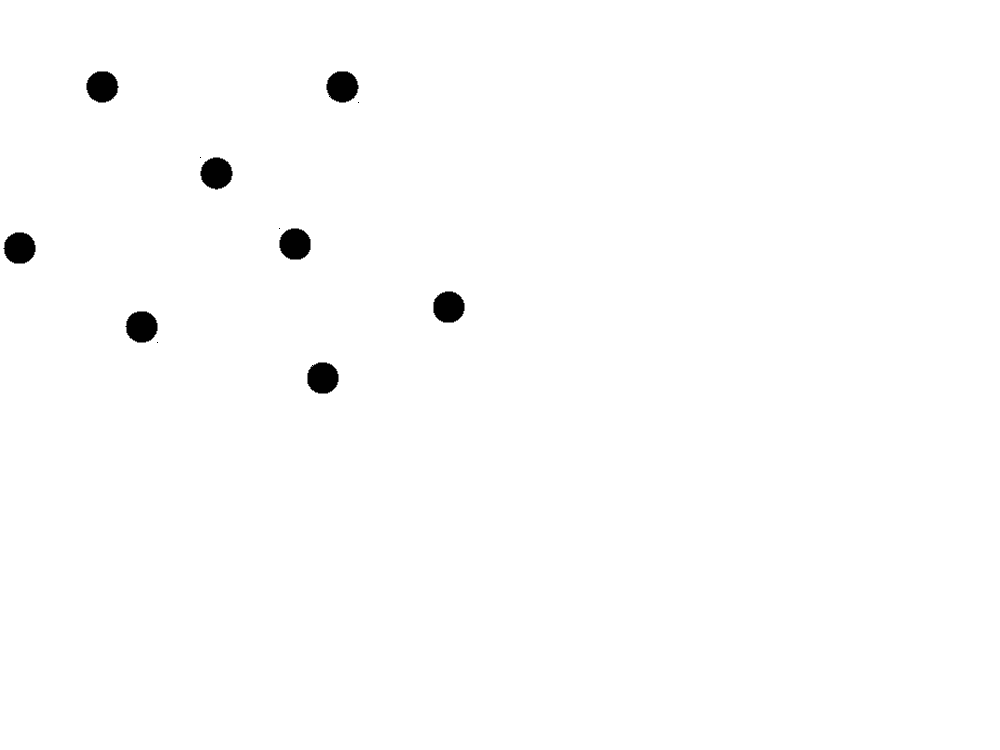
\includegraphics[width=.65\textwidth]{\fignet/FigSBM-Model-1}    
        \onslide<3>
        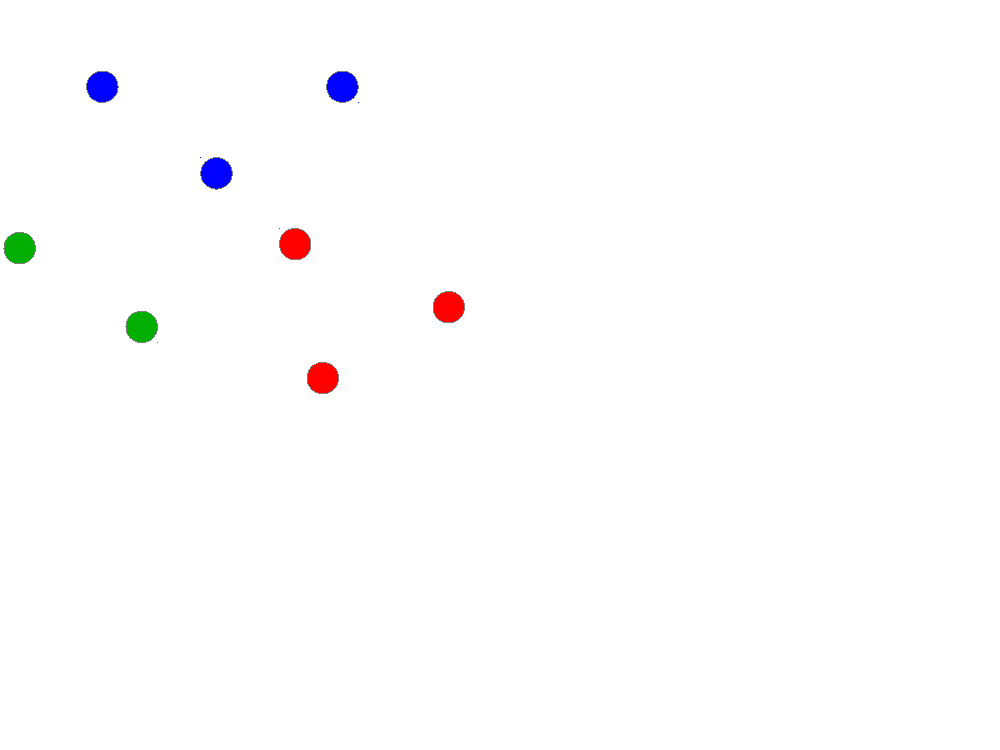
\includegraphics[width=.65\textwidth]{\fignet/FigSBM-Model-2}    
        \onslide<4>
        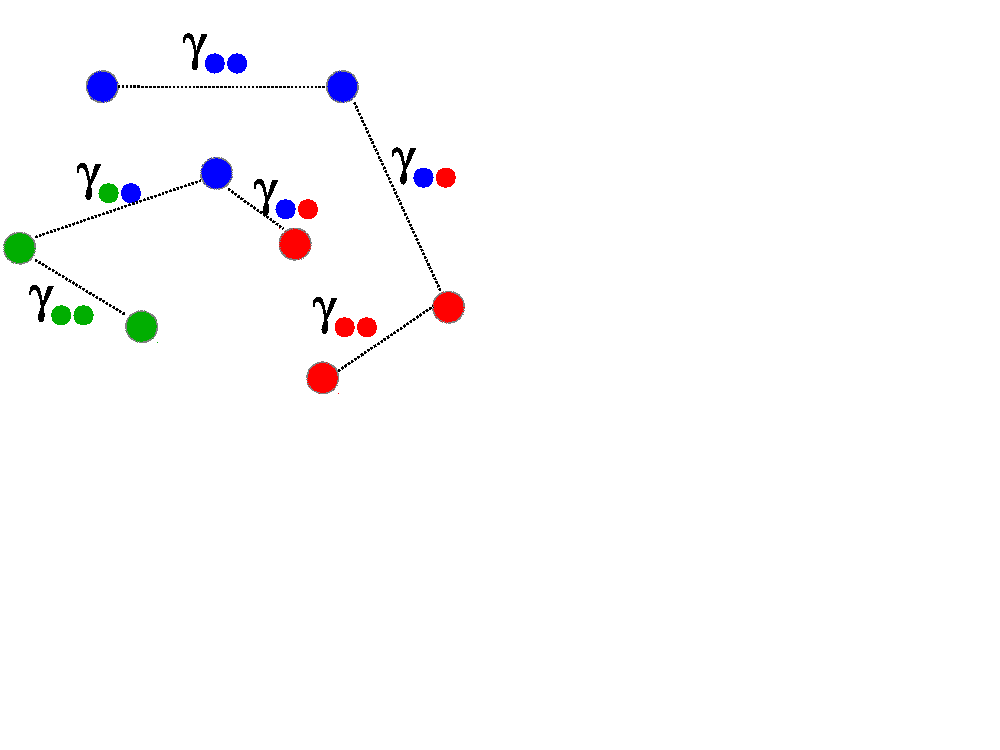
\includegraphics[width=.65\textwidth]{\fignet/FigSBM-Model-3}    
        \onslide<5>
        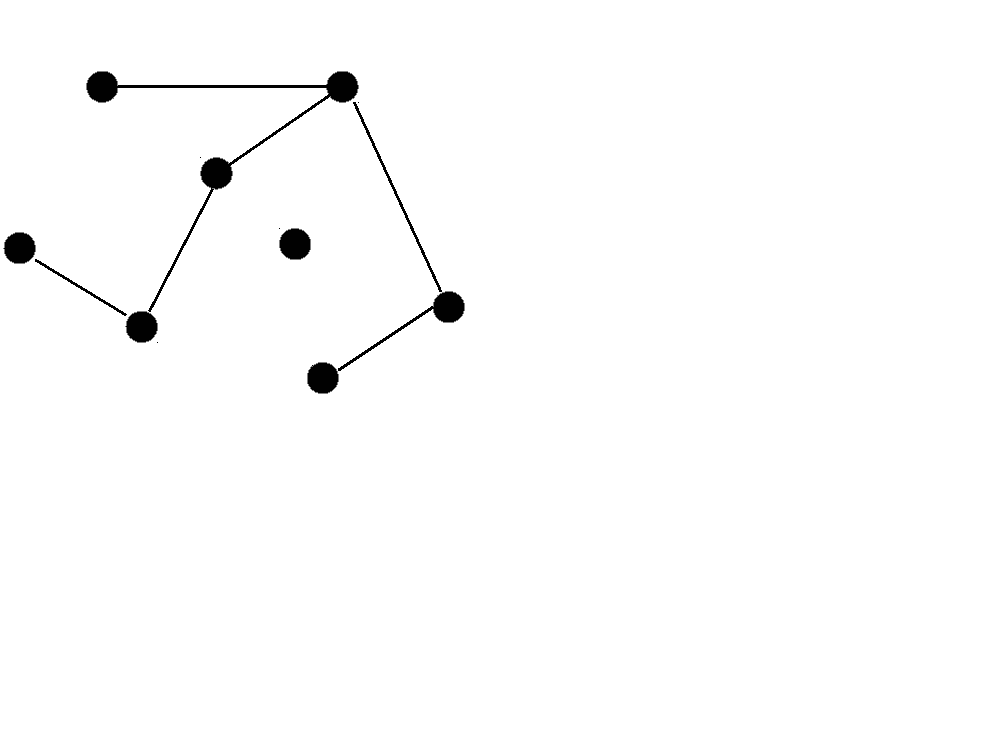
\includegraphics[width=.65\textwidth]{\fignet/FigSBM-Model-5}    
      \end{overprint}
    \end{tabular}
  \end{tabular}
  
}

%==================================================================
\frame{\frametitle{A special instance of SBM}

  \paragraph{Model.} $j, k = 1, \dots p$ nodes = species = genes, $Q$ clusters \\ ~
  \begin{enumerate}
   \item Node membership $Z_j$: each node belongs to cluster $q$ with probability $\pi_q$ \\
   \item \pause Network / GM $G$: $P\{(j, k) \in G \mid Z_j = q, Z_k = \ell\} = \gamma_{q\ell}$
   $$
   G \sim SBM_{\text{binary}}(p, \pi, \gamma)
   $$
   \item \pause Observed data: $\{Y_i\}_{i = 1, \dots n} \text{ iid } \sim \text{GM}_G$ \qquad (e.g. $Y_i \sim GGM(\Omega_G^{-1})$) \\
   \item \pause Network inference: score matrix $S = [S_{jk}] = \emphase{\text{\tt some\_network\_inference\_algorithm}}(Y)$
   $$
   (S_{jk} \mid G_{jk} = 0) \sim F_0, \qquad
   (S_{jk} \mid G_{jk} = 1) \sim F_1
   $$   
   \end{enumerate}
   
   \bigskip \pause 
   \paragraph{Assumption 2 (more questionable).} The scores $(S_{jk})$ are \emphase{independent conditionally} on the edge's existence $(G_{jk})$.
   
   \bigskip \bigskip \pause 
   \paragraph{A mixture distribution} for the edge scores:
   $$
   (S_{jk} \mid Z_j = q, Z_k = \ell) \sim (1 - \gamma_{q\ell}) F_0 + \gamma_{q\ell} F_1
   $$
}

%==================================================================
\frame{\frametitle{Inference}

  \paragraph{Aim.} Infer the parameter $\theta = (\pi, \gamma, F_0, F_1)$, the node memberships $Z = (Z_j)$ and the graph $G = (G_{jk})$.

  \bigskip \pause
  \paragraph{Incomplete data model.} 
  \begin{itemize}
   \item Neither the node memberships $Z$ nor the underlying graph $G$ are observed.
   \item The EM algorithm requires to evaluate the conditional distribution $p_\theta(Z, G \mid S)$.
  \end{itemize}

  \bigskip \pause
  \paragraph{Variational EM (VEM).} 
  \begin{itemize}
   \item Maximize a lower bound of the log-likelihood $\log p_\theta(S)$
   \item Using an approximation of the conditional distribution $p_\theta(Z, G \mid S)$:
   \begin{align*}
    \pt(Z, G) & = \pt(Z) \times \pt(G \mid Z) \\ ~ \\
    \text{where} \qquad \qquad \qquad \pt(Z) & = \prod_j \pt(Z_j) & & \text{mean field approximation} \\
    \pt(G \mid Z) & = p(G \mid Z, S) & & \text{exact form} 
%       = \underset{\text{\scriptsize mean field approximation}}{\underbrace{\prod_j \pt(Z_j)}} \times \underset{\text{\scriptsize exact form}}{\underbrace{p(G \mid Z, S)}}
   \end{align*}
  \end{itemize}
}

%==================================================================
\frame{\frametitle{Some comments}

%   \paragraph{Remarks.} \\ ~
  \begin{enumerate}    
    \item When interested in deciphering a cluster structure among species or genes, there is no need to actually infer the network (avoid a delicate thresholding step) \\ ~
    \item The observed data $Y$ do not appear in the model: the information it summarized in the score matrix $S$ \\ ~
    \item The VEM algorithm provides both
    \begin{itemize}
      \item \normalsize{the classification probabilities $\Pt\{Z_j = q\}$ for each node,} 
      \item \normalsize{as a by-product: the probability for each edge to be part of the network $\Pt\{G_{jk} = 1\}$ }
    \end{itemize} ~ \\
    \item We use Gaussian distributions for the scores: $F_0 = \Ncal(\mu_0, \sigma_0^2)$, $F_1 = \Ncal(\mu_1, \sigma_1^2)$ \\ ~
    \item $Q$ can be selected using standard (variational) $BIC$ or $ICL$ criteria. $ICL$ can account for the conditional entropy of $Z$, or $G$, or both. \\ ~
    \item Same model as \refer{RRV19}, who focus on the control of the rate of false positive edges
  \end{enumerate}
  
}

%==================================================================
\section{Simulation study}
%==================================================================
\frame{\frametitle{Simulation study}

  \bigskip
  \paragraph{Simulation design.} 
  \begin{itemize}
   \item $K = 3$ node clusters: $\pi = (17\%, 33\%, 50\%)$
   \item SBM node membership $Z$ and graph $G$: $(Z, G) \sim SBM(\pi, \gamma)$, $\overline{\gamma} = 1.5 \log(p)/p$
   \item Gaussian data $Y \sim \Ncal_p(0, \Omega_G^{-1})$
   \item Sample size $n = 20, 50, 100$
   \item Edge scores from Meinshausen-B\"uhlmann (\textcolor{red}{M-B}), \textcolor{green}{glasso}, \textcolor{blue}{tree-based} algorithms
  \end{itemize}

  \bigskip \bigskip 
  \begin{overprint}
  \onslide<2>
    \paragraph{Node classification:} ARI = adjusted rand index \\ ~
    \bigskip \bigskip 
    $\begin{array}{cccc}
    p = 20 & p = 30 & p = 50 & p = 80 \\
    \includegraphics[width=.22\textwidth]{\fignoisynetsimul/simVEM-Ktrue3-g2-K3-ARI-p20} & 
    \includegraphics[width=.22\textwidth]{\fignoisynetsimul/simVEM-Ktrue3-g2-K3-ARI-p30} &
    \includegraphics[width=.22\textwidth]{\fignoisynetsimul/simVEM-Ktrue3-g2-K3-ARI-p50} &
    \includegraphics[width=.22\textwidth]{\fignoisynetsimul/simVEM-Ktrue3-g2-K3-ARI-p80}
    \end{array}$
  \onslide<3>
  \paragraph{Edge recovery:} AUC =area under the ROC curve \\ ~
  \bigskip \bigskip
  $\begin{array}{cccc}
    p = 20 & p = 30 & p = 50 & p = 80 \\
    \includegraphics[width=.22\textwidth]{\fignoisynetsimul/simVEM-Ktrue3-g2-K3-AUC-p20} & 
    \includegraphics[width=.22\textwidth]{\fignoisynetsimul/simVEM-Ktrue3-g2-K3-AUC-p30} &
    \includegraphics[width=.22\textwidth]{\fignoisynetsimul/simVEM-Ktrue3-g2-K3-AUC-p50} &
    \includegraphics[width=.22\textwidth]{\fignoisynetsimul/simVEM-Ktrue3-g2-K3-AUC-p80}
  \end{array}$
  \end{overprint}
  
}

%==================================================================
\frame{\frametitle{Top = node classification, bottom = edge recovery}

  $
  \begin{array}{cccc}
    p = 20 & p = 30 & p = 50 & p = 80 \\
    \includegraphics[width=.22\textwidth]{\fignoisynetsimul/simVEM-Ktrue3-g2-K3-ARI-p20} & 
    \includegraphics[width=.22\textwidth]{\fignoisynetsimul/simVEM-Ktrue3-g2-K3-ARI-p30} &
    \includegraphics[width=.22\textwidth]{\fignoisynetsimul/simVEM-Ktrue3-g2-K3-ARI-p50} &
    \includegraphics[width=.22\textwidth]{\fignoisynetsimul/simVEM-Ktrue3-g2-K3-ARI-p80} \\
    ~ \\
    p = 20 & p = 30 & p = 50 & p = 80 \\
    \includegraphics[width=.22\textwidth]{\fignoisynetsimul/simVEM-Ktrue3-g2-K3-AUC-p20} & 
    \includegraphics[width=.22\textwidth]{\fignoisynetsimul/simVEM-Ktrue3-g2-K3-AUC-p30} &
    \includegraphics[width=.22\textwidth]{\fignoisynetsimul/simVEM-Ktrue3-g2-K3-AUC-p50} &
    \includegraphics[width=.22\textwidth]{\fignoisynetsimul/simVEM-Ktrue3-g2-K3-AUC-p80}
  \end{array}
  $

  Scores = \textcolor{red}{M-B}, \textcolor{green}{glasso}, \textcolor{blue}{tree}, $n = 20, 50, 100$
  
  \bigskip
  \begin{itemize}
   \item Issue with the choice of the grid of $\lambda$ in M-B and glasso
  \end{itemize}

}

%==================================================================
\section{Illustrations}
%==================================================================
\frame{\frametitle{Barents fish (1/2)}

  \paragraph{Dataset:} \refer{FNA06}
  \begin{itemize}
   \item $n = 89$ stations, $p = 30$ fish species, 
   \item $Y_{ij} =$ abundance (count) of species $j$ in station $i$, 
   \item 4 covariates (latitude, longitude, temperature and depth)
  \end{itemize}
  
  \bigskip \bigskip \pause
  \paragraph{Network inference:} 
  \begin{itemize}
   \item Fit a Poisson log-normal model \refer{AiH89} (\url{PLNmodels} package \refer{CMR18})
   \item Compute edge scores using a tree-based method (\url{EMtree} R package \refer{MRA19})
  \end{itemize}

  \bigskip \bigskip \pause
  \paragraph{Choosing the number of clusters:} $ICL(Z, G)$ criterion

}

%==================================================================
\frame{\frametitle{Barents fish (2/2)}  \label{sl:resBarents}

  \begin{tabular}{lll}
    \begin{tabular}{c}
      Choosing $Q$ \\
      \includegraphics[width=.275\textwidth]{\fignoisynetdata/BarentsFish-critTreeAll}
    \end{tabular}
    &
    \begin{tabular}{c}
      Species clusters \\
      \includegraphics[width=.275\textwidth]{\fignoisynetdata/BarentsFish-graphTreeAll}
    \end{tabular}
    &
    \begin{tabular}{c}
      Edge probabilities \\
      \includegraphics[width=.275\textwidth]{\fignoisynetdata/BarentsFish-histPsiTreeAll}
    \end{tabular} 
    \\ ~ \\
    \begin{tabular}{p{.275\textwidth}}
      \paragraph{Parameter estimates.} ~\\

      \footnotesize{$\begin{array}{rrrr}
      \multicolumn{4}{l}{\text{cluster proportions } \pi} \\
      \hline
      6.8 & 19.5 & 33.2 & 40.5 \\
      \\
      \multicolumn{4}{l}{\text{cluster connections } \gamma} \\
      \hline
      100 & 0.2 & 100 & 99.2 \\ 
      0.2 & 85.6 & 10 & 27.8 \\ 
      100 & 10 & 88.2 & 16.1 \\ 
      99.2 & 27.8 & 16.1 & 98.3 
      \end{array}$}
    \end{tabular} 
    &
    \multicolumn{2}{l}{
      \begin{tabular}{p{.6\textwidth}}
      \begin{itemize}
       \item $Q = 4$ node clusters are found, incl. one central cluster
       \item Low uncertainty for node classification \goto{sl:uncertainty}
       \item Edge probabilities are highly contrasted 
       \item The network is only drawn for an \emphase{aesthetic purpose}
      \end{itemize} 
      \end{tabular}
    }
  \end{tabular}
}

%==================================================================
\frame{\frametitle{Oak mildew (1/2)}

  \paragraph{Dataset:} \refer{JFS16}
  \begin{itemize}
   \item Metabarcoding of $p = 114$ microbial and fungal species, including the mildew pathogen {\sl E. alphitoides}
   \item Collected on $n = 116$ oak leaves
   \item $Y_{ij} =$ read count for species $j$ in leaf $i$
   \item 3 covariates (tree status, distances to ground and trunk)
  \end{itemize}
   
  \bigskip \bigskip \pause
  \paragraph{Network inference:} same procedure as for Barents fish, accounting for differential sampling depth for fungi and bacteria

}

%==================================================================
\frame{\frametitle{Oak mildew (2/2)} \label{sl:resOak}

  \begin{tabular}{lll}
    \begin{tabular}{c}
      Species correlations \\
      \includegraphics[width=.275\textwidth]{\fignoisynetdata/oaks-corrTreeAll}
    \end{tabular}
    &
    \begin{tabular}{c}
      Species clusters \\
      \includegraphics[width=.275\textwidth]{\fignoisynetdata/oaks-graphTreeAll}
    \end{tabular}
    &
    \begin{tabular}{c}
      PLNnetwork result \\
      \includegraphics[width=.275\textwidth]{\fignoisynetdata/oaks-partCorrNetTreeAll}
    \end{tabular} 
    \\ ~ \\
    \multicolumn{3}{l}{
      \begin{tabular}{p{.9\textwidth}}
      \begin{itemize}
       \item $Q = 10$ clusters found (max. value)
       \item Cluster structure in the correlation matrix (corrected for covariate effects)
       \item Consistent with direct network inference based on PLN/glasso approach \refer{CMR19}
       \item Low uncertainty for node classification \goto{sl:uncertainty}
       \item Highly contrasted edge probabilities \goto{sl:uncertainty}
       \item The pathogens \textcolor{blue}{\sl E. alphitoides} is associated with 2 fungi and 13 bacterias
      \end{itemize} 
      \end{tabular}
    }
  \end{tabular}
}

%==================================================================
\section{Discussion}
%==================================================================
\frame{\frametitle{Discussion} \label{sl:discus}

  \paragraph{To summarize.}
  \begin{itemize}
   \item A formal probabilistic framework to account for network inference uncertainty in network topology analysis via SBM
   \item An agnostic approach with respect to the network inference procedure
   \item A new instance of SBM with mixture emission distribution
   \item A VEM algorithm with $BIC$ and $ICL$ variational criteria
  \end{itemize}

  \bigskip \bigskip \pause
  \paragraph{Further work.}
  \begin{itemize}
   \item How to choose the score (i.e. the network inference method) in practice? 
   \item Non-parametric form for the score distribution \goto{sl:scoreDist}
  \end{itemize}

}

%====================================================================
\frame[allowframebreaks]{ \frametitle{References}
  {%\footnotesizen
   \tiny
   \bibliography{/home/robin/Biblio/BibGene}
%    \bibliographystyle{/home/robin/LATEX/Biblio/astats}
   \bibliographystyle{alpha}
  }
}

%==================================================================
\backupbegin

%==================================================================
\frame{\frametitle{Lasso: regularization path} \label{sl:lasso}

  \paragraph{Coefficients} become null as $\lambda$ increases
  $$
  \includegraphics[width=.4\textwidth]{\fignet/RAF-lassoPath}
  $$
  \begin{itemize}
  \item \emphase{Regularization path:} succession of optimal solutions when $\lambda$ decreases \goto{sl:scores}
  \end{itemize}
}

%==================================================================
\frame{\frametitle{Node membership and edge presence uncertainty} \label{sl:uncertainty}

  \begin{tabular}{ccc}
    \begin{tabular}{p{.15\textwidth}}
      \paragraph{Barents fish.} $Q = 4$ \\
      ~ \\
      \goto{sl:resBarents} 
    \end{tabular}
    &
    \begin{tabular}{p{.3\textwidth}}
      \includegraphics[width=.3\textwidth]{\fignoisynetdata/BarentsFish-nodeClustTreeAll} 
    \end{tabular}
    &
    \begin{tabular}{p{.3\textwidth}}
      \includegraphics[width=.3\textwidth]{\fignoisynetdata/BarentsFish-histPsiTreeAll} 
    \end{tabular}
    \\
    \begin{tabular}{p{.15\textwidth}}
      \paragraph{Oak mildew.} $Q = 9$  \\
      ~ \\
      \goto{sl:resOak} 
    \end{tabular}
    &
    \begin{tabular}{p{.3\textwidth}}
      \includegraphics[width=.3\textwidth]{\fignoisynetdata/oaks-nodeClustTreeAll} 
    \end{tabular} 
    &
    \begin{tabular}{p{.3\textwidth}}
      \includegraphics[width=.3\textwidth]{\fignoisynetdata/oaks-histPsiTreeAll} 
    \end{tabular} 
  \end{tabular}

}

%==================================================================
\frame{\frametitle{Score distribution} \label{sl:scoreDist}

  \begin{tabular}{ll}
    \begin{tabular}{p{.45\textwidth}}
      \paragraph{Barents fish.} \\
      \includegraphics[width=.4\textwidth]{\fignoisynetdata/BarentsFish-scoreDistTreeAll} \\
    \end{tabular}
    &
    \begin{tabular}{p{.45\textwidth}}
      \paragraph{Oak mildew.} \\
      \includegraphics[width=.4\textwidth]{\fignoisynetdata/oaks-scoreDistTreeAll} \\
    \end{tabular} 
  \end{tabular}

  \goto{sl:discus}
}

\backupend

%==================================================================
%==================================================================
\end{document}
%==================================================================
%==================================================================

\begin{tabular}{ll}
  \begin{tabular}{p{.45\textwidth}}
  \end{tabular}
  &
  \begin{tabular}{p{.45\textwidth}}
  \end{tabular} 
\end{tabular}
